% Options for packages loaded elsewhere
\PassOptionsToPackage{unicode}{hyperref}
\PassOptionsToPackage{hyphens}{url}
\PassOptionsToPackage{dvipsnames,svgnames*,x11names*}{xcolor}
%
\documentclass[
  a4paper,
  openany, a4paper, oneside]{book}
\usepackage{amsmath,amssymb}
\usepackage{lmodern}
\usepackage{setspace}
\usepackage{ifxetex,ifluatex}
\ifnum 0\ifxetex 1\fi\ifluatex 1\fi=0 % if pdftex
  \usepackage[T1]{fontenc}
  \usepackage[utf8]{inputenc}
  \usepackage{textcomp} % provide euro and other symbols
\else % if luatex or xetex
  \usepackage{unicode-math}
  \defaultfontfeatures{Scale=MatchLowercase}
  \defaultfontfeatures[\rmfamily]{Ligatures=TeX,Scale=1}
\fi
% Use upquote if available, for straight quotes in verbatim environments
\IfFileExists{upquote.sty}{\usepackage{upquote}}{}
\IfFileExists{microtype.sty}{% use microtype if available
  \usepackage[]{microtype}
  \UseMicrotypeSet[protrusion]{basicmath} % disable protrusion for tt fonts
}{}
\makeatletter
\@ifundefined{KOMAClassName}{% if non-KOMA class
  \IfFileExists{parskip.sty}{%
    \usepackage{parskip}
  }{% else
    \setlength{\parindent}{0pt}
    \setlength{\parskip}{6pt plus 2pt minus 1pt}}
}{% if KOMA class
  \KOMAoptions{parskip=half}}
\makeatother
\usepackage{xcolor}
\IfFileExists{xurl.sty}{\usepackage{xurl}}{} % add URL line breaks if available
\IfFileExists{bookmark.sty}{\usepackage{bookmark}}{\usepackage{hyperref}}
\hypersetup{
  pdftitle={Automated Observatory Data Curator's Handbook},
  pdfauthor={Daniel Antal, CFA},
  colorlinks=true,
  linkcolor=blue,
  filecolor=Maroon,
  citecolor=Blue,
  urlcolor=blue,
  pdfcreator={LaTeX via pandoc}}
\urlstyle{same} % disable monospaced font for URLs
\usepackage[left=2.5cm, right=2.5cm, top=2.5cm, bottom=2.5cm]{geometry}
\usepackage{longtable,booktabs,array}
\usepackage{calc} % for calculating minipage widths
% Correct order of tables after \paragraph or \subparagraph
\usepackage{etoolbox}
\makeatletter
\patchcmd\longtable{\par}{\if@noskipsec\mbox{}\fi\par}{}{}
\makeatother
% Allow footnotes in longtable head/foot
\IfFileExists{footnotehyper.sty}{\usepackage{footnotehyper}}{\usepackage{footnote}}
\makesavenoteenv{longtable}
\usepackage{graphicx}
\makeatletter
\def\maxwidth{\ifdim\Gin@nat@width>\linewidth\linewidth\else\Gin@nat@width\fi}
\def\maxheight{\ifdim\Gin@nat@height>\textheight\textheight\else\Gin@nat@height\fi}
\makeatother
% Scale images if necessary, so that they will not overflow the page
% margins by default, and it is still possible to overwrite the defaults
% using explicit options in \includegraphics[width, height, ...]{}
\setkeys{Gin}{width=\maxwidth,height=\maxheight,keepaspectratio}
% Set default figure placement to htbp
\makeatletter
\def\fps@figure{htbp}
\makeatother
\setlength{\emergencystretch}{3em} % prevent overfull lines
\providecommand{\tightlist}{%
  \setlength{\itemsep}{0pt}\setlength{\parskip}{0pt}}
\setcounter{secnumdepth}{5}
\usepackage{booktabs}
\usepackage{booktabs}
\usepackage{longtable}
\usepackage{array}
\usepackage{multirow}
\usepackage{wrapfig}
\usepackage{float}
\usepackage{colortbl}
\usepackage{pdflscape}
\usepackage{tabu}
\usepackage{threeparttable}
\usepackage{threeparttablex}
\usepackage[normalem]{ulem}
\usepackage{makecell}
\usepackage{xcolor}
\ifluatex
  \usepackage{selnolig}  % disable illegal ligatures
\fi
\usepackage[]{natbib}
\bibliographystyle{apalike}

\title{Automated Observatory Data Curator's Handbook}
\author{Daniel Antal, CFA}
\date{2021-05-16}

\begin{document}
\maketitle

{
\hypersetup{linkcolor=}
\setcounter{tocdepth}{1}
\tableofcontents
}
\listoffigures
\setstretch{1.1}
\hypertarget{introduction}{%
\chapter*{Introduction}\label{introduction}}
\addcontentsline{toc}{chapter}{Introduction}

\hypertarget{mission-statement}{%
\section*{Mission statement}\label{mission-statement}}
\addcontentsline{toc}{section}{Mission statement}

We want to win an \href{https://op.europa.eu/en/web/eudatathon}{EU Datathon prize} by processing the vast, already-available governmental and scientific open data made usable for policy-makers, scientific researchers, and business researcher end-users.

``\emph{To take part, you should propose the development of an application that links and uses open datasets. Your application should showcase opportunities for concrete business models or social enterprises. It is also expected to find suitable new approaches and solutions to help Europe achieve important goals set by the European Commission through the use of open data.}''

We want to win at least one first prize in the EU Datathon 2021.

\begin{itemize}
\tightlist
\item
  Challenge 1: \href{https://ec.europa.eu/info/strategy/priorities-2019-2024/european-green-deal_en}{A European Green Deal}, with a particular focus on the \href{https://ec.europa.eu/commission/presscorner/detail/en/ip_20_2323}{The European Climate Pact}, the \href{https://ec.europa.eu/info/food-farming-fisheries/farming/organic-farming/organic-action-plan_en}{Organic Action Plan}, and the \href{https://ec.europa.eu/commission/presscorner/detail/en/IP_21_111}{New European Bauhaus}, i.e.~mitigation strategies.
\item
  Challenge 2: \href{https://ec.europa.eu/info/strategy/priorities-2019-2024/economy-works-people_en\#:~:text=Individuals\%20and\%20businesses\%20in\%20the,needs\%20of\%20the\%20EU's\%20citizens.}{An economy that works for people}, with a particular focus on the \href{https://ec.europa.eu/info/strategy/priorities-2019-2024/economy-works-people/internal-market_en}{Single market strategy}, and particular attention to the strategy's goals of 1. Modernising our standards system, 2. Consolidating Europe's intellectual property framework, and 3. Enabling the balanced development of the collaborative economy strategic goals.
\item
  Challenge 3: \href{https://ec.europa.eu/info/strategy/priorities-2019-2024/europe-fit-digital-age_en}{A Europe fit for the digital age}, with a particular focus \href{https://ec.europa.eu/info/strategy/priorities-2019-2024/europe-fit-digital-age/excellence-trust-artificial-intelligence_en}{Artificial Intelligence}, the \href{https://ec.europa.eu/info/strategy/priorities-2019-2024/europe-fit-digital-age/european-data-strategy_en}{European Data Strategy},
  the \href{https://ec.europa.eu/info/strategy/priorities-2019-2024/europe-fit-digital-age/digital-services-act-ensuring-safe-and-accountable-online-environment_en}{Digital Services Act}, \href{https://digital-strategy.ec.europa.eu/en/policies/digital-skills-and-jobs}{Digital Skills} and \href{https://digital-strategy.ec.europa.eu/en/policies/connectivity}{Connectivity}. We will showcase these horizontal topics with our Digital Music Observatory.
\end{itemize}

For Challenge 1, we are preparing the \href{http://greendeal.dataobservatory.eu/}{Green Deal Data Observatory}.
For Challenge 2, we are preparing the \href{https://pensive-hawking-276760.netlify.app/}{Future Music Observatory} -- any better name is welcome.
For Challenge 3, we will rebrand our \href{https://music.dataobservatory.eu/}{Digital Music Observatory} to highlight our efforts in trustworthy, ethical AI, and to find a new balance between the interests of artists and music audiences.

\hypertarget{problem-statement}{%
\section*{Problem Statement}\label{problem-statement}}
\addcontentsline{toc}{section}{Problem Statement}

The EU has a 18-year-old open data regime and it makes public taxpayer-funded data in the values of tens of billions of euros per year; the Eurostat program alone handles 20,000 international data products, including at least 5000 pan-European environmental indicators.

As open science principles gain increased acceptance, scientific researchers are making hundreds of thousands of valuable datasets public and available for replication every year.

The EU, the OECD, and UN institutions run around 100 data collection programs, so-called `data observatories' that more or less avoid touching this data, and buy proprietary data instead. Annually, each observatory spends between 50 thousand and 3 million EUR on collecting untidy and proprietary data of inconsistent quality, while never even considering open data.

The problem with the current EU data strategy is that while it produces enormous quantities of valuable open data, in the absence of common basic data science and documentation principles, it seems often cheaper to create new data than to put the existing open data into shape.

This is an absolute waste of resources and efforts. With a few R packages and our deep understanding of advanced data science techniques, we can create valuable datasets from unprocessed open data. In most domains, we are able to repurpose data originally created for other purposes at a historical cost of several billions of euros, converting these unused data assets into valuable datasets that can replace tens of millions' worth of proprietary data.

What we want to achieve with this project--and we believe such an accomplishment would merit one of the first prizes--is to add value to a significant portion of pre-existing EU open data:
\href{https://data.europa.eu/data/}{data.europa.eu/data} is the new open data portal of the EU that replaces two previous versions (one for the common institutions, and technically harvesting all EU member states' national open data portals).

What we want to achieve with this project -- and we believe such an accomplishment would merit one of the first prizes -- is to add value to a significant portion of pre-existing EU open data by re-processing and integrating them into a modern, tidy database with an API access, and to find a business model that emphasises a triangular use of data in 1. business, 2. science and 3. policy-making. Our mission was to modernize the concept of `data observatories'.

\hypertarget{our-solution}{%
\section*{Our solution}\label{our-solution}}
\addcontentsline{toc}{section}{Our solution}

Recruit data curators who know how to put important policy data (according to the EU challenges) into a useful, processed format.
Help them with open-source statistical software solutions, and open-source data services to make it available for end-use in policy research (NGOs, public entities), scientific research, or business research.

Find a for-profit business model or a non-profit social enterprise model to make our service sustainable.
Contest at least 2 of the 3 Datathon challenges to show that our solution is general and not domain specific: minimally, we plan to contest the Green Deal Challenge with environmental and climate policy data, and we plan to convert our Demo Music Observatory into a Digital Music Observatory that showcases important policy issues in the Digital Life challenge.

If we were to find reliable partners in the time prior to the deadline, we would also consider submitting a bid to the third challenge, which mainly deals with economic and social policy.

Our R packages offer a professionally sound version of the data that renders it usable and reliable. In this project, we want so scale up their productivity by embedding them (and other similar packages, and even Python libraries if we can) to services.

\begin{itemize}
\tightlist
\item
  \href{https://regions.dataobservatory.eu/}{regions} corrects inconsistent geographical coding.
\item
  \href{https://iotables.dataobservatory.eu/}{iotables} puts extremely complex national accounts data into actually useful environmental and economic impact indicators.
\item
  \href{https://retroharmonize.dataobservatory.eu/}{retroharmonize} connects cross-sectional surveys with non-European countries, puts pan-European surveys into time series, and corrects regional subsamples.
\item
  indicator, in its early stage, attempts to bring to a common, tidy format the diverse and untidy indicators of European governmental open data.
\end{itemize}

The results are new statistical products, which are, in a way, a subjective interpretation of the data that is far more useful than leaving it in its original state. The usefulness of our data products is linked to our reputation, the peer-reviewed processes of our packages, and eventually, the peer-reviewed uses of the datasets created.

This means that all of our data products must possess an authentic, authored, and accountable version; therefore, all versions of our data assets are assigned Digital Object Identifiers (DOI).

For instance, if we recreate a Eurostat statistical product with corrected geocoding (member states have no mandate to correct historical data, which often results in badly-coded data), such as a new version of, say, regional CO2 emission or GDP, our version must be traceable, and eventually be available for rigorous peer-review.

\hypertarget{intro}{%
\chapter{Application for the Datathlon Prizes: Automated Data Observatories}\label{intro}}

This year's Datathlon has three challenges that we can contest with an application. We want to answer at least 2 of the challenges with the same technology, knowledge management, but partly different data used.

\hypertarget{solution-as-service-offered-in-the-challenges}{%
\section{Solution as Service offered in the Challenges}\label{solution-as-service-offered-in-the-challenges}}

\begin{itemize}
\item
  We create automated data observatories that re-process governmental and scientific open data into high-quality data that can replace better processed, but lower content value proprietary data.
\item
  We put the open data into a tidy format that allows it to be joined, and not only be used in isolation.
\item
  We fix common, simple problems, such as currency translations, unit conversions, interpolations of missing data, bad geographical coding that, without software support, makes open data not competitive.
\item
  We automate part of the documentation process, because of one of the competitive disadvantages of open data that often it is lacking any documentation.
\item
  Our automated data observatories offer re-processed, tidy and documented open data for the 2 or 3 key challenges of the EU.
\end{itemize}

\hypertarget{service-flow}{%
\section{Service Flow}\label{service-flow}}

\begin{center}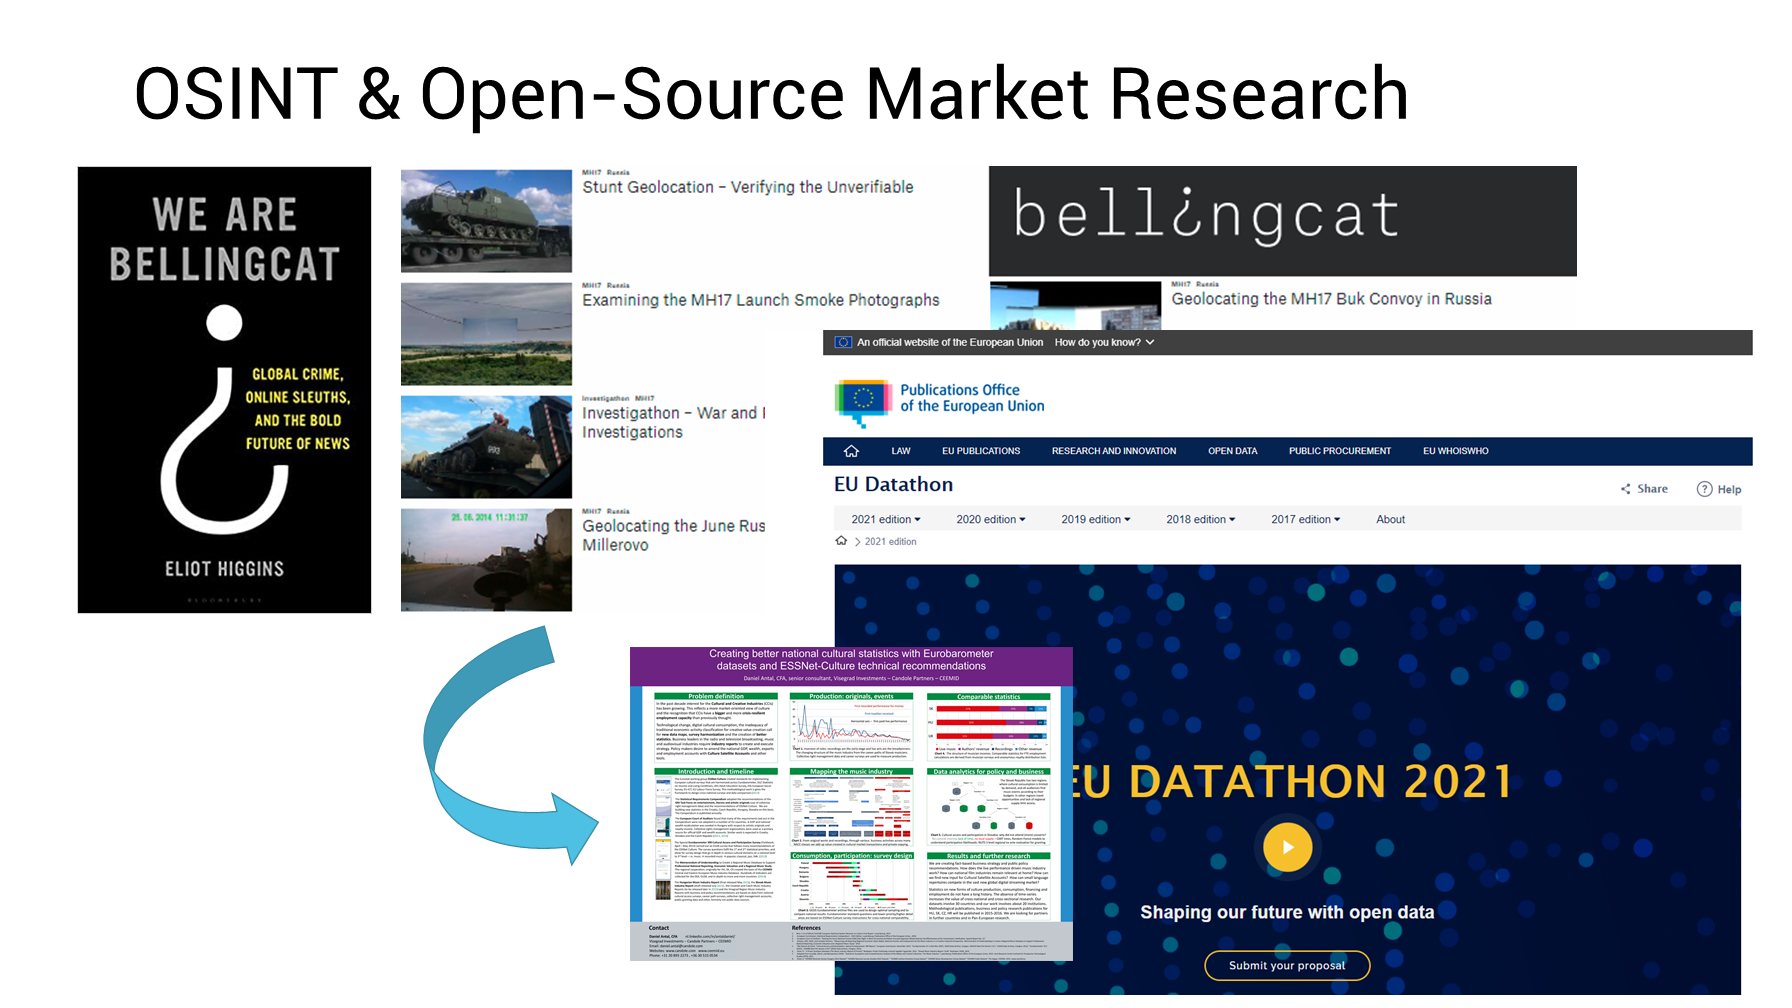
\includegraphics[width=0.8\linewidth]{plots/open_source_slide} \end{center}

\hypertarget{new-high-quality-data}{%
\subsection{New, high quality data}\label{new-high-quality-data}}

We can rely on existing packages of our team, and probably the entire rOpenGov collective, where Daniel had been active for many years. Via Kasia, we could bring in the environmental open data community.

\begin{center}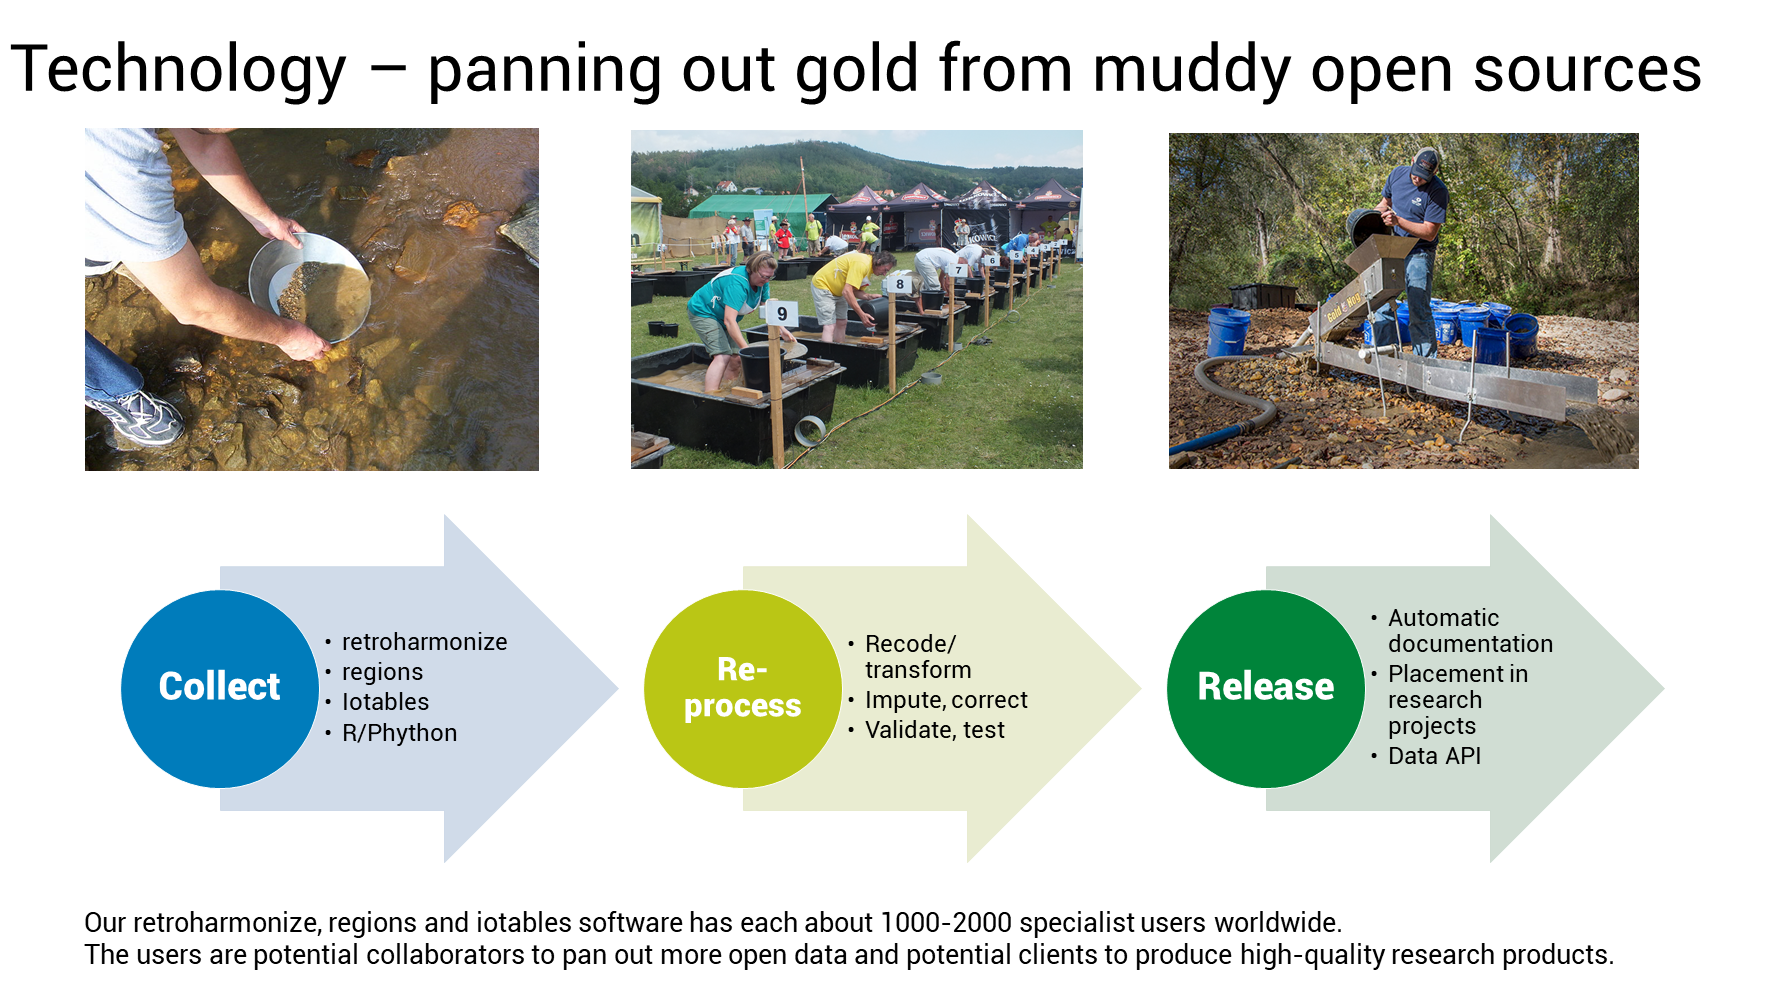
\includegraphics[width=0.8\linewidth]{plots/gold_panning_slide} \end{center}

\hypertarget{authoritative-data}{%
\subsection{Authoritative data}\label{authoritative-data}}

So, we must somehow connect to a DOI registrar, and Harvard's Dataverse or Zenodo are the candidates.

The Dataverse is much better served, the API is better documented, and technically we could even set up our own instance (new dataverses can be installed.) The problem is that I have not found an EU-endorsed instance, although Open Data Belgium has an instance. The best instance is of course the original Harvard Dataverse, but taking out European open data to an American private university would not be a winning idea. Currently Dataverse has no support on CRAN - the R package was just kicked out of CRAN, and it is buggy, but it can be fixed.

Zenodo is a semi-endorsed EU solution, originating from CERN, and in the last EU budget period all EU-funded research was supposed to deposit data there. The API is far less documented. Manual deposition is working fine, and we can very easily retrieve our own data in various versions. It is also free data storage. But communicating with the API is a challenge. In R, Zen4R is supposed to be on CRAN, but extremely ill-documented, and uses a special R6 class which is beyond the level and practicality of 99\% R users. It seems that it is very well supported in Python, though.

\hypertarget{data-api}{%
\subsection{Data API}\label{data-api}}

We have settled for Datasette, which is powering the John Hopkins Covid database, for example. It is a lightweight, Python-based application that turns a Sqlite database into a powerful API. Botond has set up our first instances and we are very happy with the results.

\begin{center}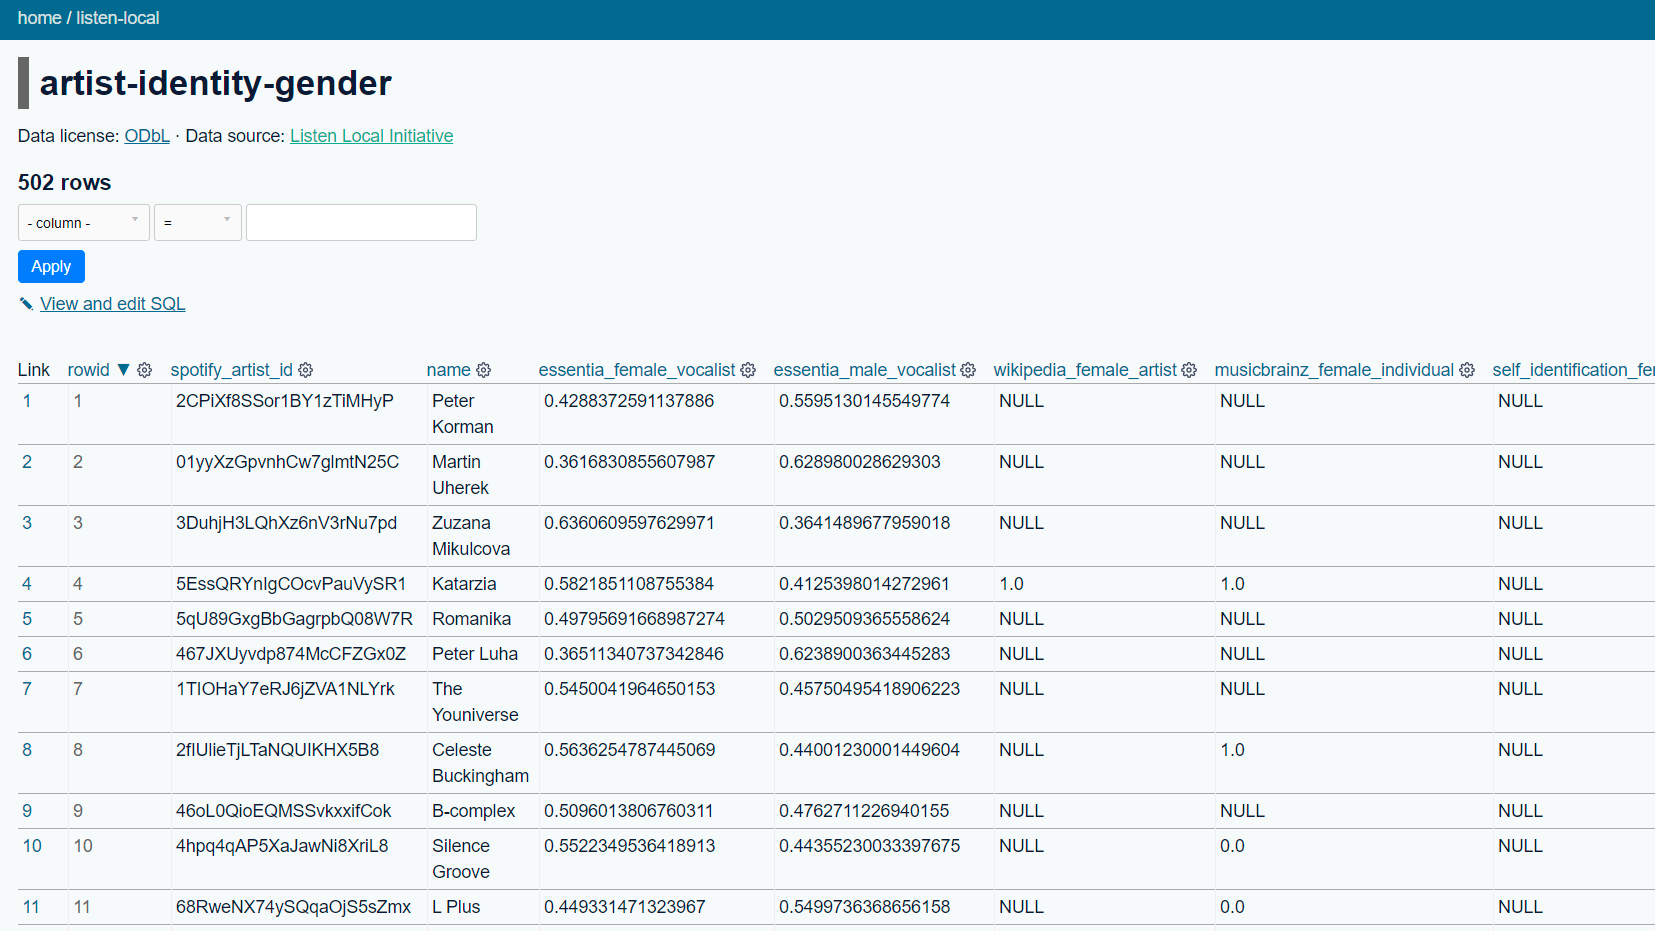
\includegraphics[width=0.8\linewidth]{plots/data-api-artist-gender-table} \end{center}

\hypertarget{long-form-documentation}{%
\subsection{Long form documentation}\label{long-form-documentation}}

Our long-form documentation is based in R rmarkdown, knitr, and bookdown. It is a very mature workflow, it produces a long-form website, and PDF, ePUB or Word versions.

We take the data from our Data API / Zenodo, describe it and visualize it as it changes.

\hypertarget{front-end-website}{%
\subsection{Front-end Website}\label{front-end-website}}

We create a front-end website to present our curators, recruit new ones, blog about great new use cases, in a hugo website.

Our website needs a chief editor, and hugo website operations manager.

The current websites are powered by a hugo template, formerly known as academic, currently as wowchemy academic.The idea was that an offspring of bookdown, i.e.~blogdown can integrate this hugo technology into an R workflow. This is a semi-success, and while academic is a super-popular template, it is getting further and further away from blogdown. The original advantage that it can be managed in the same workflow as the indicator generation, package documentation, the long-form documentation is a bit gone.

\begin{center}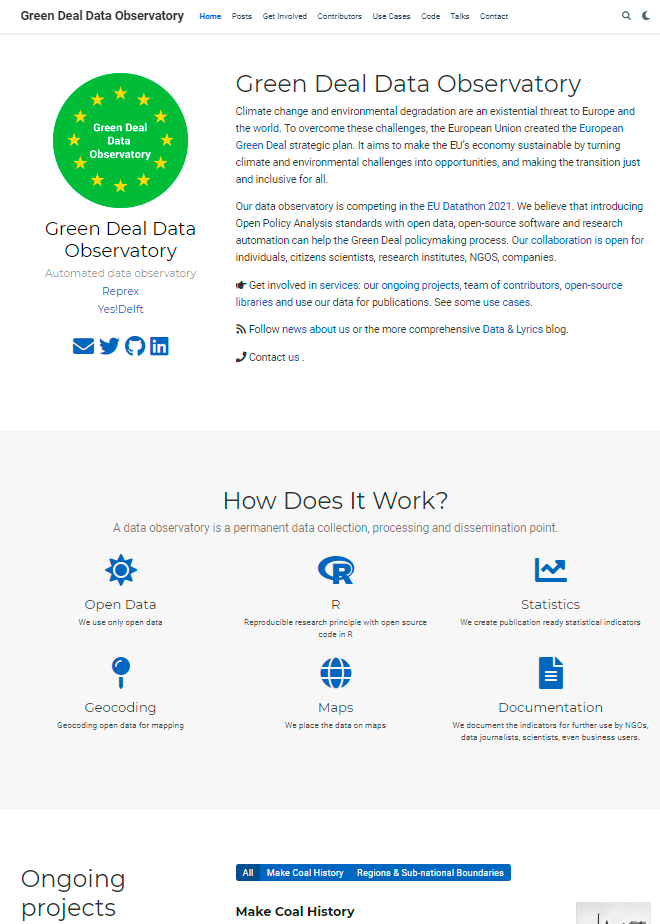
\includegraphics[width=0.8\linewidth]{plots/green_deal_hugo} \end{center}

\hypertarget{technology}{%
\section{Technology}\label{technology}}

Peer-reviewed R packages on CRAN, and potentially peer-reviewed Python libraries which attest that our new datasets are sound from a (1) processing point of view.
Help with R/ Python code, tutorials our curators to create well-documented, authored open datasets, and deposit them on Zenodo (preferred) or Harvard Dataverse.\\
Each observatory will maintain a ``Zenodo community'' where we also take in any other related data via our curators, and we give authenticated copies of our data with DOIs.
We make our data available in a neat Datasette API. The Datasette API should harvest the data from several points (with low-frequency data, from Zenodo, as it will be in synch with the DOI versions; with high frequency data, the other way around: every month we should make a DOI versioned authentic copy of the high-frequency data from a Datasette dump)
We create via Rmarkdown / bookdown an automated, long-form documentation to all our datasets, including, when applicable, maps or visualizations.
This workflow can incorporate seaborne visualizations from the Datasette, too, but the visualization effort should be comfortable for both R and Python-based curators.
We create a hugo website as a frontend to each observatory to present our curators, recruit new ones, blog about great new use cases, in a hugo website. These are our current ones, but it would be nice to have a hugo manager who takes it over from Daniel \url{https://greendeal.netlify.app/}, \url{https://music.dataobservatory.eu/} {[}we'll completely overhaul this{]}

\hypertarget{data-curators}{%
\chapter{Data Curators}\label{data-curators}}

We are looking for data curators who

\begin{enumerate}
\def\labelenumi{\arabic{enumi}.}
\tightlist
\item
  Work with governmental or scientific or otherwise \protect\hyperlink{open-data}{open data}.
\item
  Committed to high policy or business professional standards, and by making their work \protect\hyperlink{reproducible-research}{reproducible}, they adhere to reviewability, reproducability, confirmability and auditability, regardless if they work, or study for various professsional roles in business, academia, public or non-governmental policy, and data journalism.
\item
  They are interested in helping us with \protect\hyperlink{indicator-design}{indicator design}.
\item
  Make the authoritative copy of their indicator available on the Zenodo data repository, and keep it up-to-date with our automated observatory's help.
\end{enumerate}

\begin{quote}
An important aspect of the EU Datathon Challenges is ``.. to propose the development of an application that links and uses open datasets {[}\ldots{]} to find suitable new approaches and solutions to help Europe achieve important goals set by the European Commission through the use of open data.''
\end{quote}

\hypertarget{open-data}{%
\section{Open Data}\label{open-data}}

In the EU, open data is governed by the \href{https://eur-lex.europa.eu/legal-content/EN/TXT/?qid=1561563110433\&uri=CELEX:32019L1024}{Directive on open data and the re-use of public sector information - in short: Open Data Directive (EU) 2019 / 1024}. It entered into force on 16 July 2019. It replaces the \href{https://eur-lex.europa.eu/legal-content/en/ALL/?uri=CELEX:32003L0098}{Public Sector Information Directive}, also known as the \emph{PSI Directive} which dated from 2003 and was subsequently amended in 2013.

\hypertarget{reproducible-research}{%
\section{Reproducible Research}\label{reproducible-research}}

\textbf{Reproducible research} is a scientific concept that can be applied to a wide range of professional designations. We are applying this concept to \protect\hyperlink{opa}{Evidence-based, Open Policy Analysis} and \protect\hyperlink{business-professional-standards}{Professional Standards in Business}.

for example, reproducible finance in the investment process or reproducible impact assessment in policy consulting. Based on the computational reproducibility we believe that the following principles should be followed.

\begin{itemize}
\item
  \textbf{Reviewability} means that our application's results are can be assessed and judged by our user's experts, or experts they trust. We help reviewability with full transparency: we publish the software code that created the indicators, our methodology, and an automatically refreshing statistical description of the indicator each day when it receives new data or corrections from the original source.
\item
  \textbf{Reproducibility} means that we are providing data products and tools that allow the exact duplication of our results during assessments. This ensures that all logical steps can be verified. Reproducibility ensures that there is no lock-in to our applications. You can always chose a different data and software vendor, or compare our results with them.
\item
  \textbf{Confirmability} means that using our applications findings leads to the same professional results as other available software and information. Our data products use the open-source statistical programming language R. We provide details about our algorithms and methodology to confirm our results in SPSS or Stata or sometimes even in Excel.
\item
  \textbf{Auditability} means that our data and software is archived in a way that external auditors can later review, reproduce and confirm our findings. This is a \emph{stricter form of data retention} that most organizations apply, because we do not only archive results step-by-step but all computational steps -- as if your colleagues would not only save every step in Excel but also their keystrokes. While auditability is a requirement in accounting, we are extending this approach to all the quantitative work of a professional organization in an advisory or consulting capacity.
\item
  \textbf{Reviewable findings}: The descriptions of the methods can be independently assessed, and the results judged credible. In our view, this is a fundamental requirement for all professional applications. CEEMID's music data is used to settle royalty disputes in judicial procedures, or in grant and policy design. We believe that the future European Music Observatory should aim at the same bar, making its data \& research products open for challenges in the publicity of science, courts, and professional peers.
\item
  \textbf{Replicable findings}: We are presenting our findings and provide tools so that our users or auditors or external authorities can duplicate our results.
\item
  \textbf{Confirmable findings}: The main conclusions of the research can be obtained independently without our software, because we describe in detail the algorithms and methodology in supplementary materials. We believe that other organizations, analysts, statisticians must come to the same findings with their own methods and software. This avoids lock-in and allows independent cross-examination.
\item
  \textbf{Auditable findings}: Sufficient records (including data and software) have been archived so that the research can be defended later if necessary or differences between independent confirmations resolved. The archive might be private, as with traditional laboratory notebooks. See \protect\hyperlink{opencollaboration}{Open collaboration} with academia, auditors, and industry.
\end{itemize}

These computational requirements require a data workflow that relies on further principles.

\begin{itemize}
\item
  \textbf{Record retention}: all aspects of reproducibility require a high level of standardized documentation. The standardization of documentation requires the use of standardized metadata, metadata structures, taxonomies, vocabularies.
\item
  \textbf{Best available information / data universe}: the quality of the findings, their confirmation and auditing success will improve with better data and facts used.
\item
  \textbf{Data validations}: The quality of the findings will greatly depend on the factual inputs. While the reproducible findings may have many problems, inputting erroneous data or faulty information will likely lead to wrong conclusions, and in all cases will make confirmation and auditing impossible. Especially when organizations use large and heterogeneous data sources, even small errors, such as erroneous currency translations or accidental misuse of decimals, units can cause results that will not pass confirmation or auditing.
\end{itemize}

\hypertarget{opa}{%
\subsection{Evidence-based, Open Policy Analysis}\label{opa}}

In the last two decades, governments and researchers have placed a growing emphasis on the value of evidence-based policy. However, while the evidence generated through research to inform policy has become more rigorous and transparent, policy analysis--the process of contextualizing evidence to inform specific policy decisions--remains opaque.

We believe that a modern data observatory must improve how evidence is created and used in policy reports, and pass on the efficiency gains from increasing reproducibility and automation. Therefore, we pledge that the \href{https://music.dataobservatory.eu}{music.dataobservatory.eu} will comply with the \href{https://www.bitss.org/opa/}{Open Policy Analysis} standards developed by the \href{https://www.bitss.org/}{Berkeley Initiative for Transparency in the Social Sciences} \& \href{https://cega.berkeley.edu/}{Center for Effective Global Action}. These standards are applied by the World Bank.

\hypertarget{business-professional-standards}{%
\subsection{Professional Standards in Business}\label{business-professional-standards}}

Some of the requirements of reproducible research are usually required by professional standards. For example, various accounting, finance, legal or consulting professional standards call for appropriate documentation and record retention.

\hypertarget{indicator-design}{%
\section{Indicator Design}\label{indicator-design}}

We are committing ourselves in the final deliverable to follow the indicator design principles set out by Eurostat:
\citep{eurostat_harmonised_indicators_2014, kotzeva_harmonised_indicators_2017, eurostat_harmonised_indicators_2014} to create high-quality, validated indicators that receive appropriate feedback from users, i.e.~music businesses, their trade associations and policy-makers.

Examples for indicators in our \href{https://music.dataobservatory.eu/}{Digital Music Observatory}:

\begin{itemize}
\item
  Indicators that were used with all known royalty valuation methods \citep{pwc_valuing_2008}, for both author's and neighbouring rights, and fullfil the \href{https://www.ifrs.org/issued-standards/list-of-standards/ifrs-13-fair-value-measurement/}{IFRS fair value} standards, incorporated in \href{https://eur-lex.europa.eu/legal-content/EN/TXT/HTML/?uri=CELEX:32012R1255\&from=EN\%7D}{EU law} and the recent EU jurisprudence \citep{cjeu_osa_2014, cjeu_akka_2017}.
\item
  Indicators that can be used for calculating damages, or calculating the value of the value gap \citep{antal_pcr_croatia_2019, antal_szabad_2019_en}.
\item
  Indicators that quantify the development needs of musicians, and can set objective granting aims and grant evaluations \citep{antal_javaslatok_2015}.
\item
  Understanding how music is taxed, how music contributes to the local and national GDP, and how music creates jobs directly, indirectly and with induced effects \citep{antal_slovenskom_hudobnom_2019}.
\item
  Providing detailed comparison of the differences of music audience among countries.
\item
  Measuring exporting success on streaming platforms, and preparing better targeting tools.
\end{itemize}

\hypertarget{authoring-indicator}{%
\subsection{Creation and Quality Control of Indicators}\label{authoring-indicator}}

An indicator values are created if we the data curator has some, preferably at least 20 observation values available in data table that confirms the tidy data principles, i.e.~each variable is in exactly one column of the table, and each observation is in one row of the table.

Each indicators should be described in a clear, English language text, describing the meaning of the variables, the source of the observations, and other important information about the processing, refreshing, extending of the dataset.

We are safeguarding the quality of the indicators with various reproducible research methods. Depending on the data scientific level of the curator, we either take over the quality control mechanism, or cooperate with the curator. But the main inputs for quality control should be described by the data curator.

\begin{itemize}
\item
  \textbf{Unit testing}: Unit tests are simple, numerical test that avoid logical errors in an indicator. Shall we exclude zero values? Negative values? Do percentages must add up to 100? Some of our indicators go through more than 60 unit tests. We ask your help to get us going, and we will take care of the usual suspects: wrong currency translations, wrong decimal places (thousand, million units), etc.
\item
  \textbf{Missing data treatment}: No real life dataset is complete, but many statistical and AI methods cannot handle missing values. Therefore, we make an effort to \emph{impute} with an estimated value the missing values. Imputation is sometimes self-understanding, but sometimes it is a very tricky business, particularly when the data has several dimensions (particularly time or geographical dimension.) We want to agree with the curator why some data may be missing, and how best to handle it. For simple, two dimensional datasets, by default, we use linear approximation, forecasting and backcasting of the values, and in small datasets the last observation carry forward or the next observation carry backwards methods. May compromise the data? Let us know.
\item
  \textbf{Testing against peer-reviewed results}: Often we know that after making various computations with a data, we must achieve an already known value. For example, the various components of the GDP in economics must add up with a pre-defined precision. Certain inputs must match a scientifically valid result. If you know of such tests, let us know, and let's include them in the unit-testing processes.
\item
  \textbf{Peer-reviewed data manipulation code}: Whenever we re-organize, impute, or otherwise change the original data, we do it only with algorithms that went through scientific peer-review as algorithms. If there is a bug or something to improve in the way we handle the data, our code transparency makes it likely to come out.
\item
  \textbf{Peer-reviewed data application}: We encourage our curators, particularly academics, to send the indicators created with the help of oour research automation to various forms of scientific peer review, to make sure that the data is valid, useful\ldots{} and to bring credits to the curators.
\item
  \textbf{Authentic copies}: We are placing each new version of the indicators values into \href{https://zenodo.org/}{Zenodo}, a data repository that keeps authentic copies, versions, and assignes them digital object identifiers (DOIs). This makes sure that whenever our curators data is re-used, and incorrectly manipulated by a business, scientific or policy user, we can detect such manipulation.
\end{itemize}

\begin{figure}

{\centering 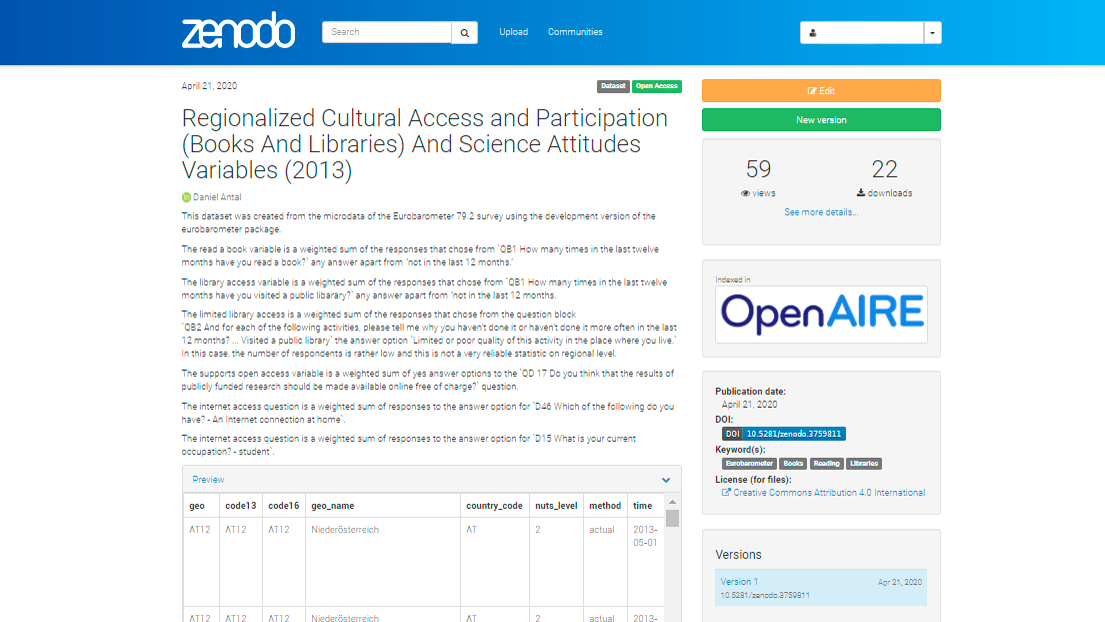
\includegraphics[width=0.8\linewidth]{plots/screenshots/zenodo_deposition_example} 

}

\caption{Zenodo Deposition Example}\label{fig:zenodo-example}
\end{figure}

You can see this dataset \href{https://zenodo.org/record/3759811\#.YJ6R3qgzbIU}{here}, which was used in \href{https://dataandlyrics.com/publication/scholarly_pirate_libraries_2020/}{this} high-profile scientific publication.

\hypertarget{deposit-indicator}{%
\subsection{Authentic Depositions of Indicators}\label{deposit-indicator}}

We designed a workflow that helps our curators to put their indicator tables to \href{https://zenodo.org/}{Zenodo}. In many cases, particularly if they do EU-funded research, this is also usually a grant requirement. At the same time, we place the indicator to our database, and make it available on our data observatory's API.

With low-frequency data, such as annual data tables, we place all copies to Zenodo first, and then to the data API. In these cases, each new version of the indicator values (containing a new year, a new estimation, or a new country, a new observation unit) will have a new DOI version.

With high-frequency data, such as data tables that are refreshing daily or several times a day, we do not think that authentic versioning is useful. In such cases, we create an authentic version at a pre-agreed time frequency, for example, monthly.

\hypertarget{your-first-data-contribution}{%
\section{Your First Data Contribution}\label{your-first-data-contribution}}

Your first contribution can be made without writing a single program code -- but if you are experienced in reproducible science, than you can also submit a code that creates your data.

\begin{enumerate}
\def\labelenumi{\arabic{enumi}.}
\item
  Make sure that you read the \href{https://www.contributor-covenant.org/}{Contributors Covenant}. You must make this \href{https://www.contributor-covenant.org/version/2/0/code_of_conduct/}{pledge} to make participation in our community a harassment-free experience for everyone, regardless of age, body size, visible or invisible disability, ethnicity, sex characteristics, gender identity and expression, level of experience, education, socio-economic status, nationality, personal appearance, race, caste, color, religion, or sexual identity and orientation. Participating in our data observatories requires everybody to act and interact in ways that contribute to an open, welcoming, diverse, inclusive, and healthy community. It's better this way for you and for us!
\item
  Send us a plain language document about the indicator. What should the indicator be used for, how it should be measured, with what frequency, and what could be the open data source to acquire the observations. Experienced data scientists can send us a Jupiter Notebook or an Rmarkdown file with code, but this submission can be a simple plain language document without numbers.
\item
  Make sure that you have and \href{https://orcid.org/}{ORCiD ID}. This is a standard identification for scientific publications. We need your numeric ORCiD ID.
\item
  Make sure that you have a \href{https://zenodo.org/}{Zenodo account} which is connected to your \href{https://orcid.org/}{ORCiD ID}. This enables you to publish data under your name. If you curate data for our observatories, you will be the indicator's first author, and depending on what processes help you, the author of the (scientific) code that helps you calculate the values will be your co-author.
\item
  Without programming experience your first indicator should be uploaded manually to Zenodo, and we will help automating the new versions. This will mean, for example, the upload of a simple, csv version of an Excel table, and filling in some important information about the contents of the table.
\item
  With some level of R or Python programming experience, we ask you to create a Github repo where you store your indicator. We will help you with tutorials, program codes, or applications to automate your data publication on Zenodo. In this case, make sure that you also have a \href{https://sandbox.zenodo.org/}{Sandbox Zenodo} account. There is no undo button on Zenodo. If you are tinkering with automatically publishing data, practice first in the sandbox, which is a practicing clone of Zenodo with undo button. (To avoid accidents, you need to have a completely different account with different credential on the real and the sandbox practice repository.)
\item
  Experienced programmers are welcome to participate in our developer team, and become contributors, or eventually co-authors of the (scientific) software codes that we make to continuously improve our data observatories. All our data code is open source. At this level, you are expected to be able to raise and/or pick up and solve an issue in our observatory's Github repository, or its connecting statistical repositories.
\end{enumerate}

\emph{Our data is mainly processed in R language software, and sometimes in Python language software. If you are experienced with R bookdown, R Shiny or working in the hugo language, then you are welcome to join our developer team in non-curatorial roles.}

\hypertarget{green-deal}{%
\chapter{Green Deal Indicators}\label{green-deal}}

Climate change and environmental degradation are an existential threat to Europe and the world. To overcome these challenges, the European Union created the European Green Deal strategic plan. It aims to make the EU's economy sustainable by turning climate and environmental challenges into opportunities, and making the transition just and inclusive for all.

Our data observatory is competing in the EU Datathon 2021. We believe that introducing Open Policy Analysis standards with open data, open-source software and research automation can help the Green Deal policymaking process. Our collaboration is open for individuals, citizens scientists, research institutes, NGOS, companies.

\begin{center}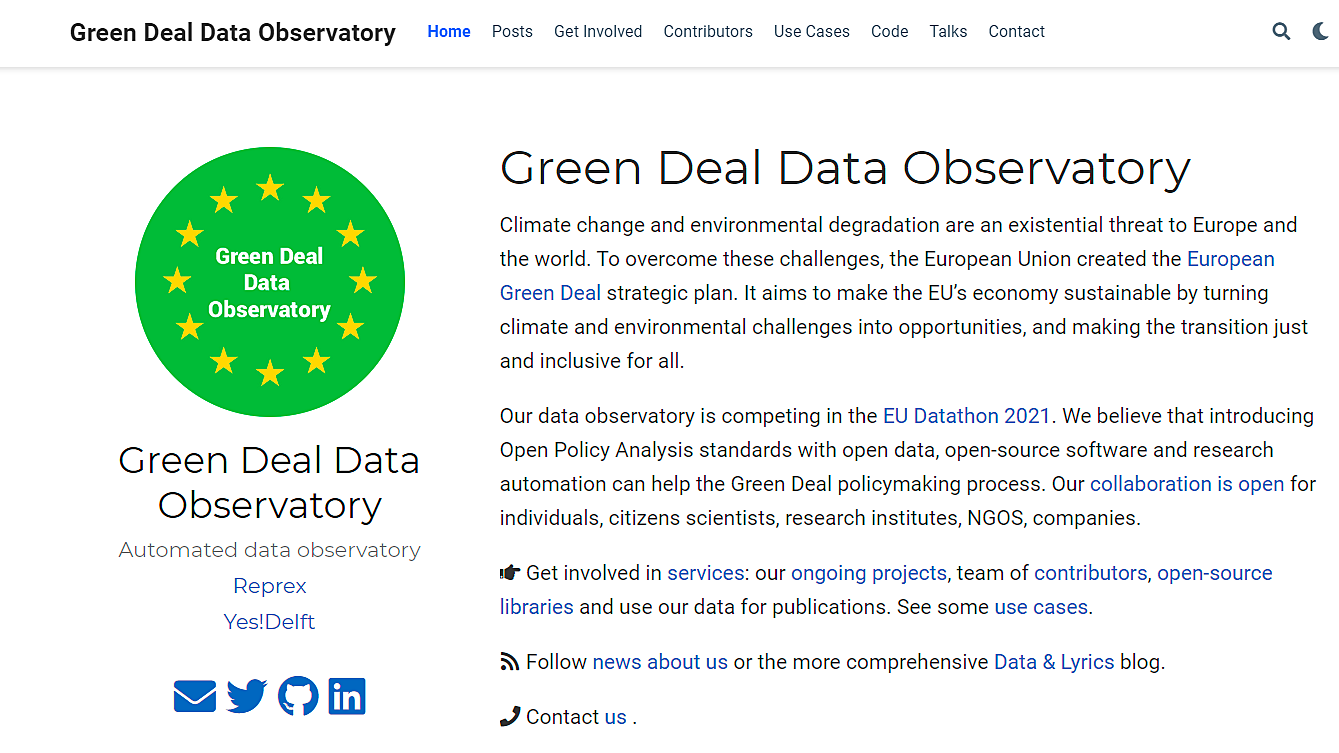
\includegraphics[width=0.8\linewidth]{plots/green_deal_observatory} \end{center}

\hypertarget{social-attituted-to-climate-change}{%
\section{Social Attituted to Climate Change}\label{social-attituted-to-climate-change}}

what do people think about climate change in Europe and other parts of the world? Do they believe that the climate is changing? How? What they think about the causes? Do they report that they change their behavior? Teach their children to do so?

Please take a look at our blogpost \href{http://greendeal.dataobservatory.eu/post/2021-04-23-belgium-flood-insurance/}{Is Drought Risk Uninsurable?} as an example.

As a data curator:

\begin{itemize}
\tightlist
\item
  You identify openly accessible surveys that are harmonized (use standardized questions.) In our tutorial we projected the public opinion data from Eurobarometer 90.2 (fieldwork: October-November 2018.) on the municipal map of Belgium
\item
  Tell us which question items would be good candidates to report. We used the answers to the multiple choice question \texttt{QB1\ Do\ you\ think\ that\ the\ following\ extreme\ weather\ events\ are\ due\ to\ climate\ change?} We highlighted areas where people find it more likely to be exposed to \texttt{Droughts\ and\ wildfires}
\item
  How we should calculate the indicator? Take a certain answer and average it over a region? Weight the answers? How?
\item
  You write at least 1-2 unit tests: what must we check when the calculation is over. No negative numbers? Number of regions must up to 265?
\end{itemize}

If you write R code, you can get involved in our suvey harmonization and regional coding efforts.

See our tutorial:

\href{http://greendeal.dataobservatory.eu/post/2021-03-06-regions-climate/}{Regional Geocoding Harmonization Case Study - Regional Climate Change Awareness Datasets}

\begin{figure}

{\centering 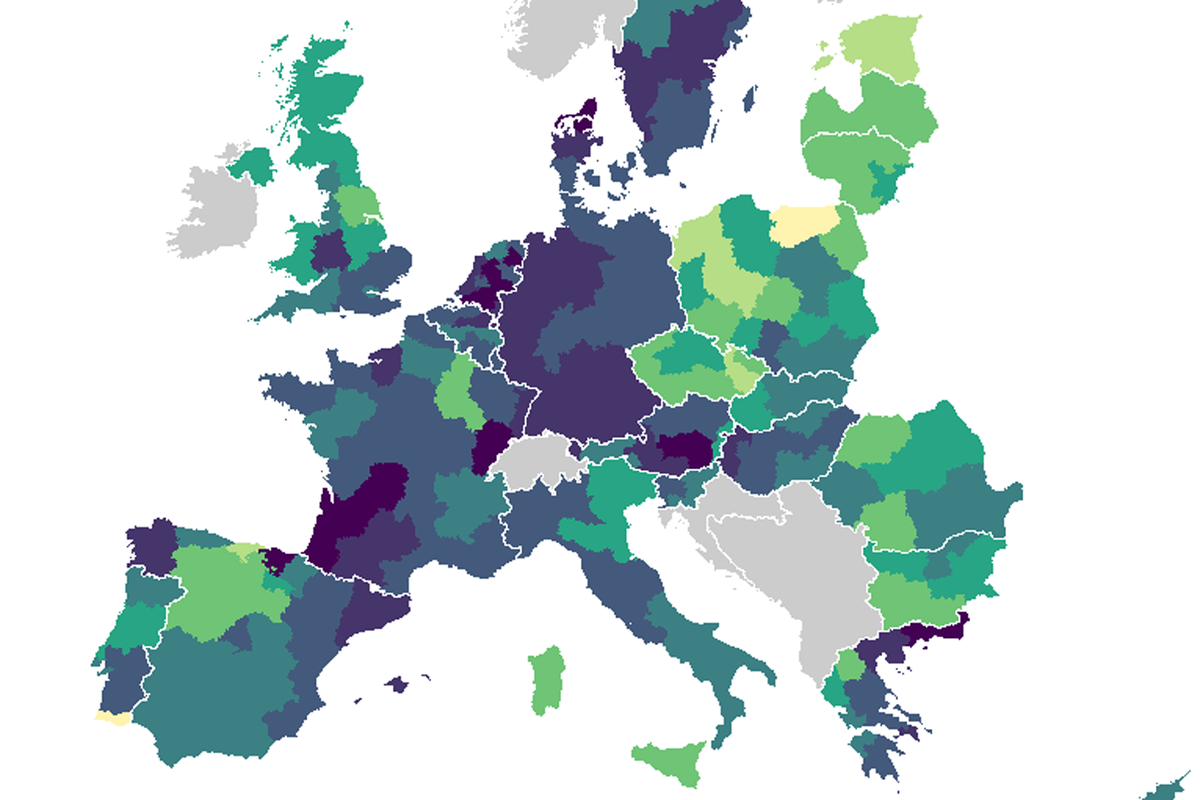
\includegraphics[width=0.67\linewidth]{plots/eurobarometer_climate_attitude_tutorial} 

}

\caption{Regional attituteds to climate change, from our survey regionalization tutorial}\label{fig:regional-climate-attitutes-tutorial}
\end{figure}

\hypertarget{environmental-impact-indicator-for-economic-activities}{%
\section{Environmental Impact Indicator for Economic Activities}\label{environmental-impact-indicator-for-economic-activities}}

Our \href{https://iotables.dataobservatory.eu/}{iotables} package practically implements The \href{https://ec.europa.eu/eurostat/en/web/products-manuals-and-guidelines/-/KS-RA-07-013}{Eurostat Manual of Supply, Use and Input-Output Tables} with real life data and in R, and it is checked against the published results from \href{http://ec.europa.eu/eurostat/documents/3859598/5902113/KS-RA-07-013-EN.PDF/b0b3d71e-3930-4442-94be-70b36cea9b39?version=1.0}{Jörg Beutel} (the author of this excellent manual), the Spicosa Project Report, and official UK statistical tables.

We used it to calculate the effects of cultural activities on various economies, but this methodology is particularly well-suited to measure the effects, or predict the effects of policy changes on greenhouse gas or pollutant emissions.

As a data curator:

\begin{itemize}
\tightlist
\item
  You identify openly accessible surveys data that can contains environmental effects for industries (Eurostat publishes them for many pollutants and greenhouse gases from the European Environmental Data.)
\item
  Tell us which particular data table would be good candidate to report. Give us ideas how to bridge various problems. (The SIOT matrix must be 60x60 or 64x64), sometimes industries must be added together.
\item
  If you write R code, we help you make the calculation yourself, if not, we'll take over.\\
\item
  Please assess the results with us, and let's publish them regularly. (Some EU member states update their SIOTs every year, others every 5 years, but pollutant data may be available annually.)
\end{itemize}

\hypertarget{sensory-data-measuring-climate-change-physical-affects}{%
\section{Sensory Data Measuring Climate Change Physical Affects}\label{sensory-data-measuring-climate-change-physical-affects}}

\hypertarget{ecological-data}{%
\section{Ecological Data}\label{ecological-data}}

\hypertarget{future-economy}{%
\chapter{Future Economy Observatory}\label{future-economy}}

Big data and automation create new inequalities and injustices and has a potential to create a jobless growth. Our Economy Observatory is a fully automated, open source, open data observatory that produces new indicators from open data sources and experimental big data sources, with authoritative copies and a modern API.

Our observatory is monitoring the European economy to protect the consumers and the small companies from unfair competition both from data and knowledge monopolization and robotization. We take a critical SME-, intellectual property policy and competition policy point of view automation, robotization, and the AI revolution on the service-oriented European social market economy.

We would like to create early-warning, risk, economic effect, and impact indicators that can be used in scientific, business and policy contexts for professionals who are working on re-setting the European economy after a devastating pandemic and in the age of AI. We are particularly interested in designing indicators that can be early warnings for killer acquisitions, algorithmic and offline discrimination against consumers based on nationality or place of residence, signs of undermining key economic and competition policy goals, and generally help small and medium-sized enterprises and start-ups to grow, and the financial sector to provide loanable and equity funds for their growth.

\begin{center}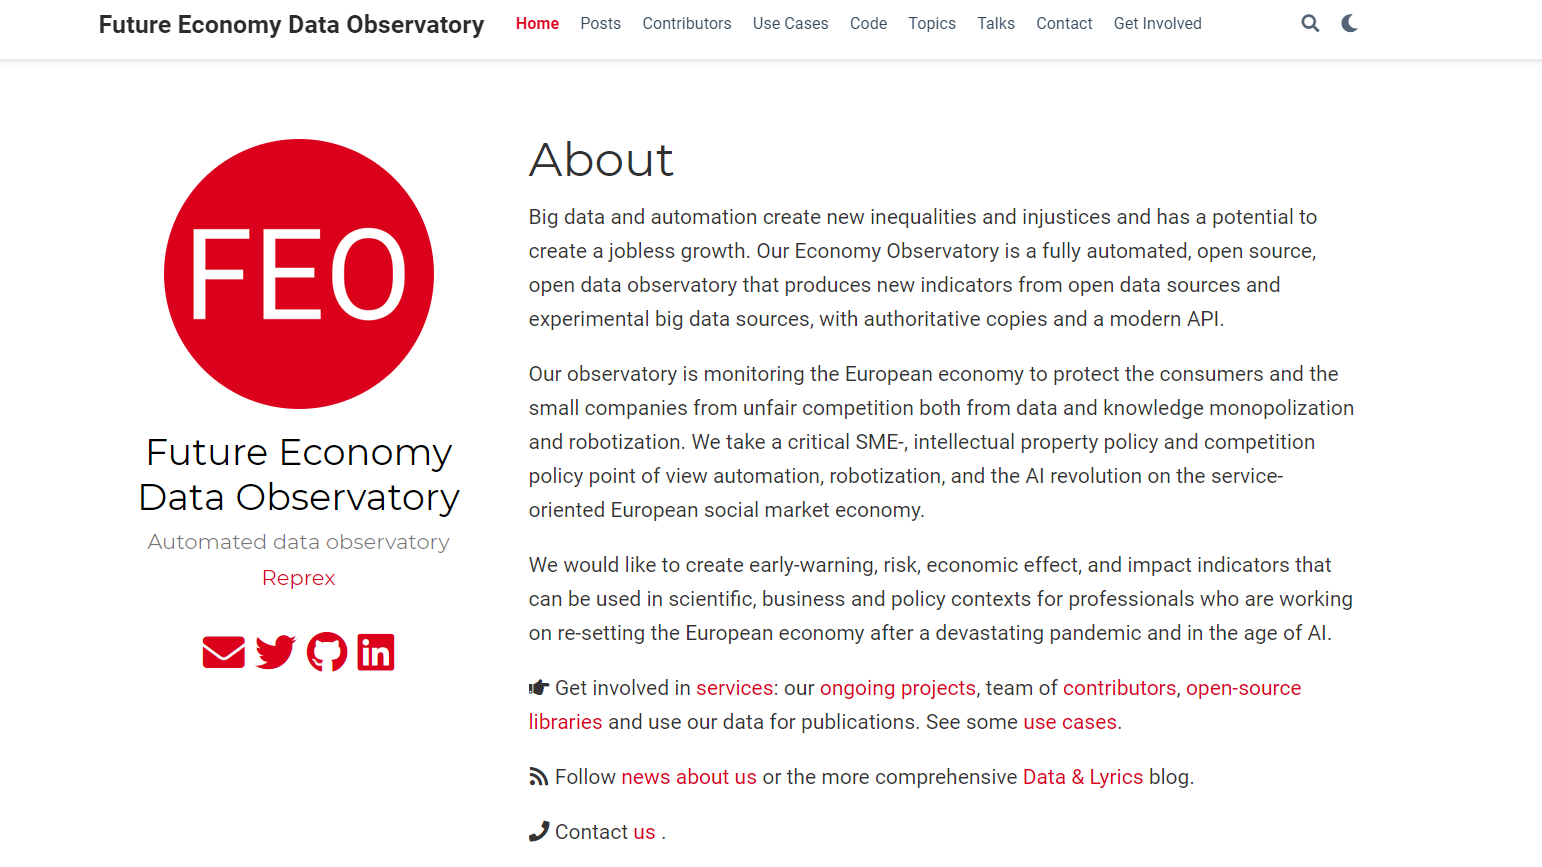
\includegraphics[width=0.8\linewidth]{plots/screenshots/fmo_screenshot} \end{center}

\begin{quote}
An important aspect of the EU Datathon Challenges is ``.. to propose the development of an application that links and uses open datasets {[}\ldots{]} to find suitable new approaches and solutions to help Europe achieve important goals set by the European Commission through the use of open data.''
\end{quote}

In the \href{https://ec.europa.eu/info/strategy/priorities-2019-2024/economy-works-people_en\#:~:text=Individuals\%20and\%20businesses\%20in\%20the,needs\%20of\%20the\%20EU's\%20citizens.}{An economy that works for people} challenge we are focusing on the \href{https://ec.europa.eu/info/strategy/priorities-2019-2024/economy-works-people/internal-market_en}{Single market strategy}, and particular attention to the strategy's goals of 1. Modernising our standards system, 2. Consolidating Europe's intellectual property framework, and 3. Enabling the balanced development of the collaborative economy strategic goals.

\hypertarget{social-attitutes-to-economic-change}{%
\section{Social Attitutes to Economic Change}\label{social-attitutes-to-economic-change}}

what do people think about climate change in Europe and other parts of the world? Do they believe that the climate is changing? How? What they think about the causes? Do they report that they change their behavior? Teach their children to do so?

Please take a look at our blogpost \href{http://greendeal.dataobservatory.eu/post/2021-04-23-belgium-flood-insurance/}{Is Drought Risk Uninsurable?} as an example.

As a data curator:

\begin{itemize}
\tightlist
\item
  You identify openly accessible surveys that are harmonized (use standardized questions.) In our tutorial we projected the public opinion data from Eurobarometer 90.2 (fieldwork: October-November 2018.) on the municipal map of Belgium
\item
  Tell us which question items would be good candidates to report. We used the answers to the multiple choice question \texttt{QB1\ Do\ you\ think\ that\ the\ following\ extreme\ weather\ events\ are\ due\ to\ climate\ change?} We highlighted areas where people find it more likely to be exposed to \texttt{Droughts\ and\ wildfires}
\item
  How we should calculate the indicator? Take a certain answer and average it over a region? Weight the answers? How?
\item
  You write at least 1-2 unit tests: what must we check when the calculation is over. No negative numbers? Number of regions must up to 265?
\end{itemize}

If you write R code, you can get involved in our suvey harmonization and regional coding efforts.

See our tutorial:

\href{http://greendeal.dataobservatory.eu/post/2021-03-06-regions-climate/}{Regional Geocoding Harmonization Case Study - Regional Climate Change Awareness Datasets}

\begin{figure}

{\centering 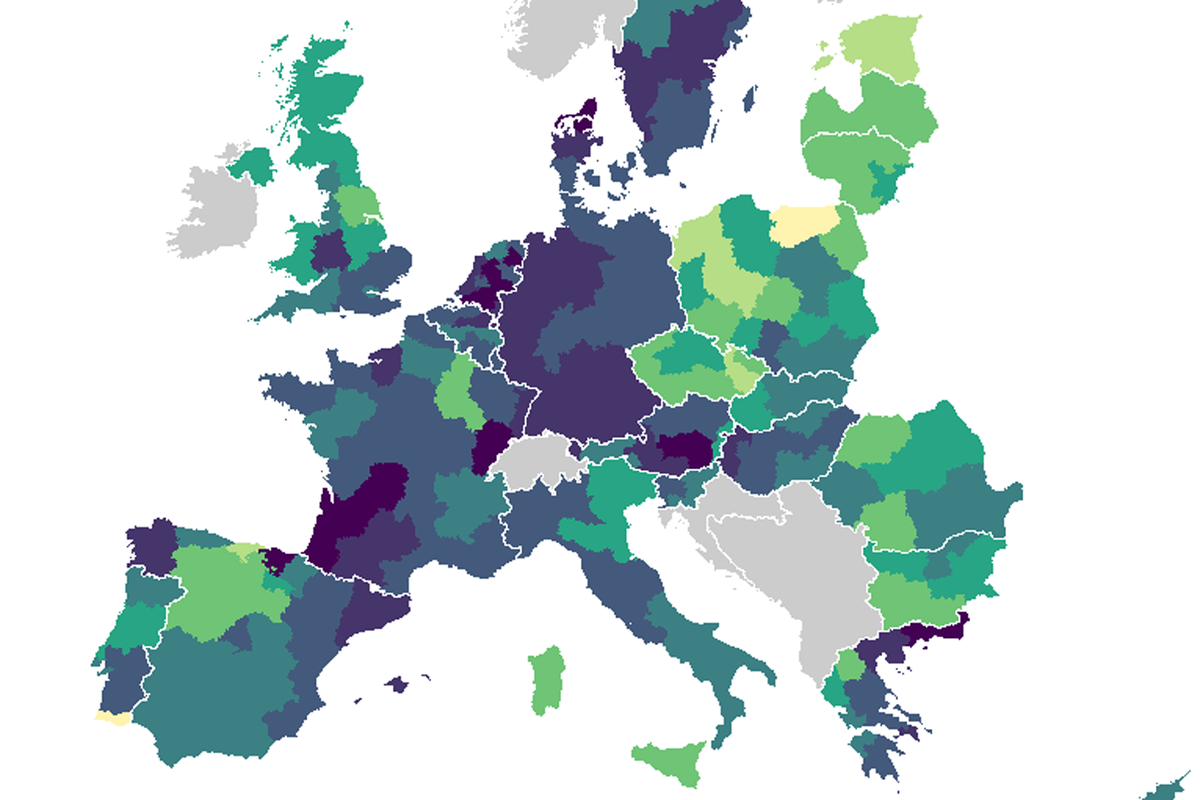
\includegraphics[width=0.67\linewidth]{plots/eurobarometer_climate_attitude_tutorial} 

}

\caption{Regional attituteds to climate change, from our survey regionalization tutorial}\label{fig:regional-climate-attitutes-tutorial-2}
\end{figure}

\hypertarget{compeition-indicators}{%
\section{Competition}\label{compeition-indicators}}

We are seeking API level access to the European Commissions Mergers database, and monitor approved and declined merger requests programatically. These mergers are important cases enough to have a potential impact on the structure of the European economy.

\begin{figure}

{\centering 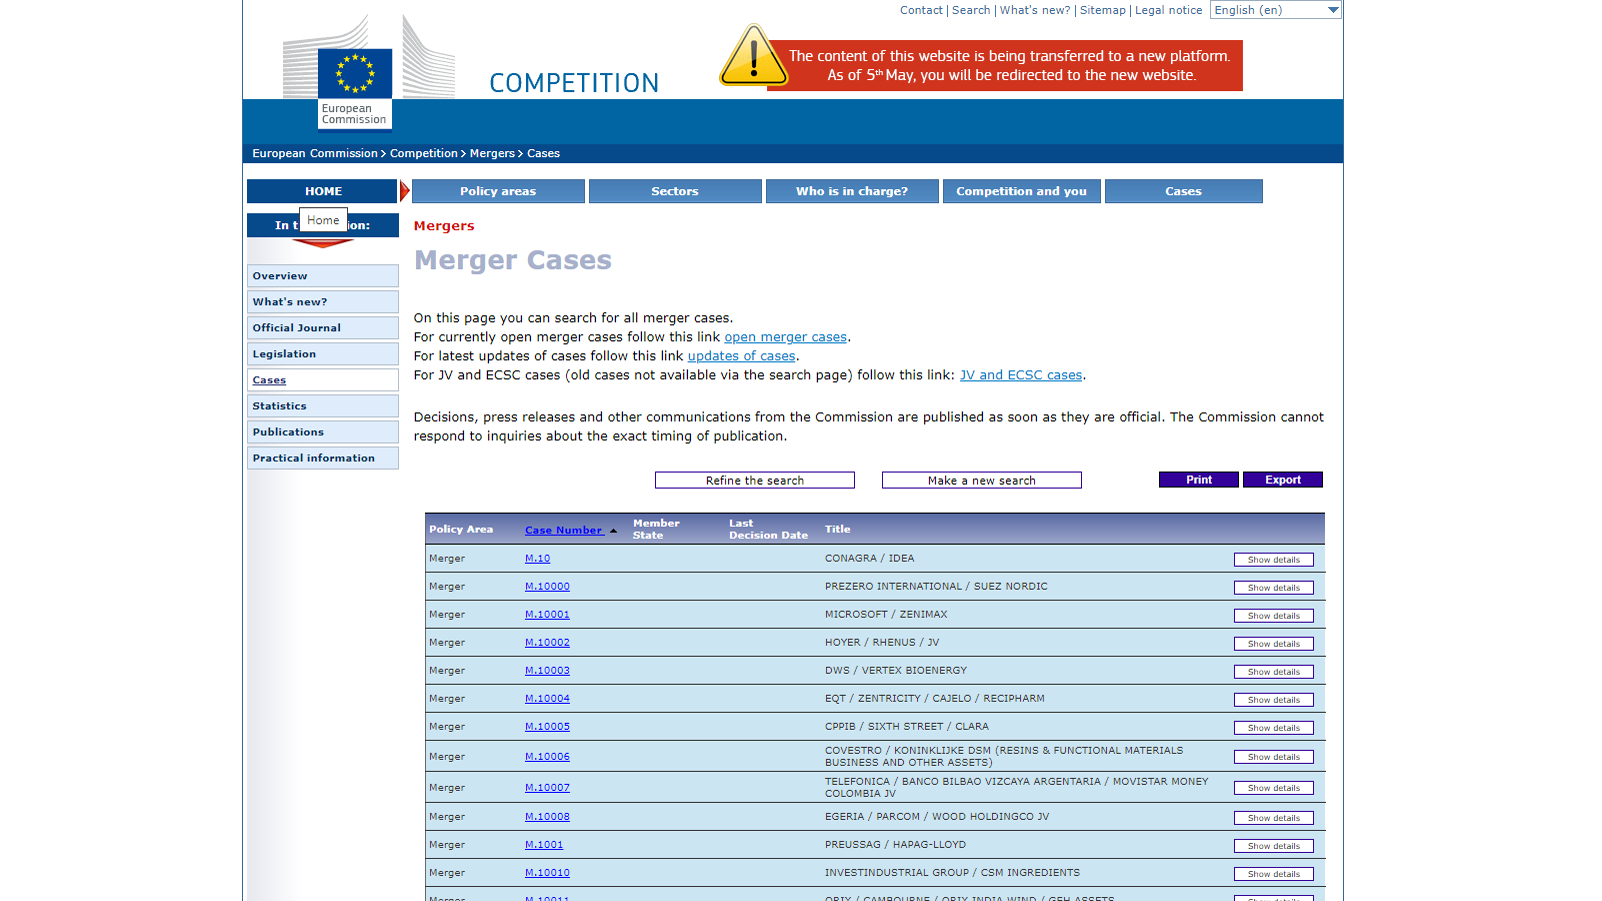
\includegraphics[width=0.8\linewidth]{plots/screenshots/ec_competition_merger_screenshot} 

}

\end{figure}

As a data curator, you help us designing datasets

\begin{itemize}
\tightlist
\item
  created from Commission and member state merger decision text databases (we will use NLP extraction from the text of the decisions)
\item
  top-down indicators that show the structural (concentration) changes in the European economy
\item
  connect them to patent databases
\end{itemize}

These indicators are particularly interestign, because we are trying to connect to databases that fall under the \href{https://eur-lex.europa.eu/legal-content/EN/TXT/?qid=1561563110433\&uri=CELEX:32019L1024}{Directive on open data and the re-use of public sector information - in short: Open Data Directive (EU) 2019 / 1024}, but programmatic access appears to be problematic. We need to secure reproducible, programmatic access to these important open data sources.

\hypertarget{knowledge-monopoly}{%
\subsection{Knowledge Monopolizations, Killer Acquisitions}\label{knowledge-monopoly}}

In killer acquisitions, a large company, for example, in pharmaceutical or technology fiedls, buys a small company, or even a start-up, to avoid disruptive innovation. We are building several types of indicators in this field.

\begin{itemize}
\tightlist
\item
  What type of patents companies hold in smaller entities of mergers and acquisitions? How can we characterize potentially disruptive technology?
\item
  Which economic activities (industries as describe by NACE) are more and less effected?
\item
  How is patent concentration changing?
\end{itemize}

\hypertarget{sme-indicators}{%
\section{SME Activity Indicators}\label{sme-indicators}}

\hypertarget{economic-impact-indicators}{%
\section{Economic Impact Indicators}\label{economic-impact-indicators}}

Our \href{https://iotables.dataobservatory.eu/}{iotables} package practically implements The \href{https://ec.europa.eu/eurostat/en/web/products-manuals-and-guidelines/-/KS-RA-07-013}{Eurostat Manual of Supply, Use and Input-Output Tables} with real life data and in R, and it is checked against the published results from \href{http://ec.europa.eu/eurostat/documents/3859598/5902113/KS-RA-07-013-EN.PDF/b0b3d71e-3930-4442-94be-70b36cea9b39?version=1.0}{Jörg Beutel} (the author of this excellent manual), the Spicosa Project Report, and official UK statistical tables.

We used it to calculate the effects of cultural activities on various economies, but this methodology is particularly well-suited to measure the effects, or predict the effects of policy changes on greenhouse gas or pollutant emissions.

As a data curator:

\begin{itemize}
\tightlist
\item
  You identify openly accessible surveys data that can contains environmental effects for industries (Eurostat publishes them for many pollutants and greenhouse gases from the European Environmental Data.)
\item
  Tell us which particular data table would be good candidate to report. Give us ideas how to bridge various problems. (The SIOT matrix must be 60x60 or 64x64), sometimes industries must be added together.
\item
  If you write R code, we help you make the calculation yourself, if not, we'll take over.\\
\item
  Please assess the results with us, and let's publish them regularly. (Some EU member states update their SIOTs every year, others every 5 years, but pollutant data may be available annually.)
\end{itemize}

\hypertarget{sensory-data-measuring-changes-in-economic-activy}{%
\section{Sensory Data Measuring Changes in Economic Activy}\label{sensory-data-measuring-changes-in-economic-activy}}

\hypertarget{music-data}{%
\chapter{Music Data Indicators}\label{music-data}}

The Digital Music Observatory (DMO) is a fully automated, open source, open data observatory that links public datasets in order to provide a comprehensive view of the European music industry. While the current music ecosystem provides European consumers with ease of access, its effects on artists and creative businesses have been devastating. The DMO produces key business and policy indicators that enable the growth of music business strategies and national music policies in a way that works both for music lover audiences and the creative enterprises of the sector.

Music is one of the most data-driven service industries where the majority of sales are already made by AI-driven autonomous systems. We provide a template that enables making these AI-driven systems accountable and trustworthy, with the goal of re-balancing the legitimate interests of creators and consumers. Music, like all creative industries, can create high-value, human jobs in the future that utilize digital skills and human creativity. Within Europe, this new balance will be an important use case of the European Data Strategy and the Digital Services Act.

The DMO places the values of the European Data Strategy at its center: our observatory model allows the seamless flow of data within the EU and across sectors; it abides by European rules concerning privacy, access, and use; it pools data from a wide range of industries and sectors and makes it available for further research. The music industry is a global industry, and the best known European music scene in the world is the British. Our observatory aims to support a new relationship between the European and the UK music industries while offering international open data products from global sources.

The DMO is a fully-functional service that can function as a testing ground of the European Data Strategy, showcasing the ways in which the music industry is affected by the problems that the Digital Services Act and European Trustworthy AI initiatives attempt to regulate. Our observatory's policy insights also shed new light on important aspects of the Digital Skills and Connectivity agenda of the European Union. As a user-friendly one-stop shop for all things concerning data and the music industry, our DMO provides the foundations for a healthier and accountable European music ecosystem.

\begin{center}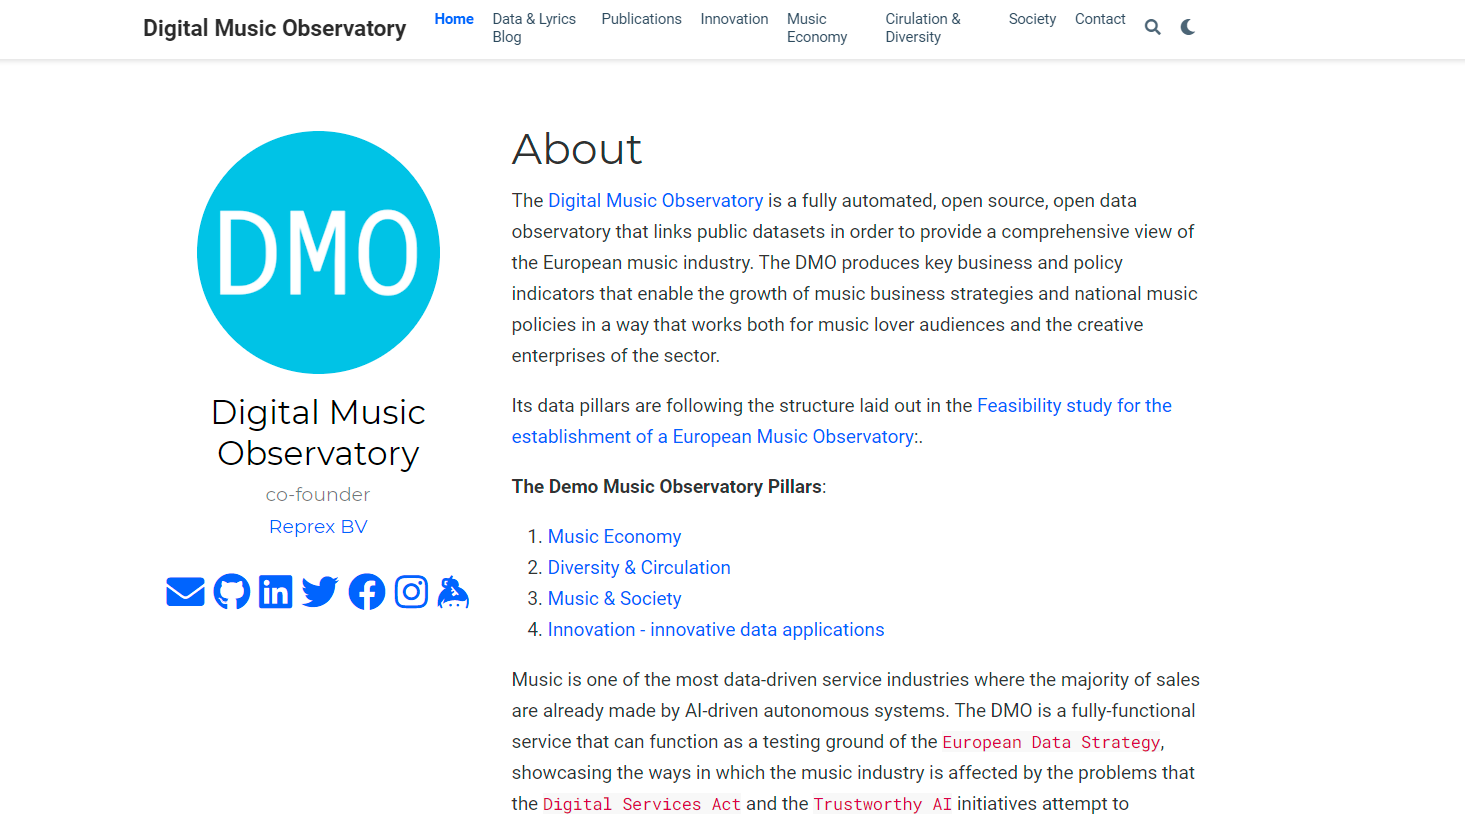
\includegraphics[width=0.8\linewidth]{plots/dmo_opening_page} \end{center}

\hypertarget{music-economy}{%
\section{Music Economy}\label{music-economy}}

\hypertarget{demand-drivers}{%
\subsection{Demand Drivers}\label{demand-drivers}}

Our music economy \href{https://data.music.dataobservatory.eu/music-economy.html}{demand drivers} are data that are known to be leading indicators to an increase in mechanical copies, streaming subscriptions, public performance use, private copying or illegal use of music.

\hypertarget{supply-indicators}{%
\subsection{Supply Indicators}\label{supply-indicators}}

Our Music Economy / \href{https://data.music.dataobservatory.eu/music-economy.html\#supply}{Supply} indicators are related to the supply of new music.

\hypertarget{price-indicators}{%
\subsection{Price Indicators}\label{price-indicators}}

\hypertarget{music-diversity}{%
\section{Music Diversity}\label{music-diversity}}

\hypertarget{gender-language-ethnic-and-other-inclusion-attributes}{%
\subsection{Gender, Language, Ethnic and Other Inclusion Attributes}\label{gender-language-ethnic-and-other-inclusion-attributes}}

\hypertarget{music-circulation}{%
\section{Music Circulation}\label{music-circulation}}

\hypertarget{market-shares}{%
\subsection{Market shares}\label{market-shares}}

We are developing \href{https://data.music.dataobservatory.eu/music-diversity.html\#cross-border-circulation-of-works}{market share} indicators for streaming and broadcast music.

For national, gender or other market share, we need to label both music works and recorded fixations. We use various open source databases, and machine learning algorithms to do prepare the data, but eventually our data goes through human musicology or music journalist curators.

For example, in our case study we were interested in the various definitions of \texttt{Slovak\ market\ share}, and representation of \texttt{female\ artists.} Both problems require rather challenging labeling.

\begin{enumerate}
\def\labelenumi{\alph{enumi})}
\tightlist
\item
  we tried to find a location to the artist / band {[} you can describe why this is not always straightforward, for example, in the case of dead artists, etc.{]}
\item
  our algorithm tried to guess the language of the 10 most popular song titles
\item
  we checked if the person is on the Wikipedia list of ``Slovak male singers'', ``Slovak female singers'', ``Slovak bands'', or their Czechoslovak versions {[} who did you decide when somebody was Czechoslovak if they were Slovak{]}
\item
  check if there was a Slovak placename mentioned on their bandcamp site
\item
  check if they are associated with Slovakia on the Musicbrainz open source database
\item
  if any of the artists released recodings was released in Slovakia
\item
  if the majority of the artist's released recordings was released in Slovakia
\end{enumerate}

\ldots.

Until we got to the human curation.

and eventually we either \texttt{considered\_slovak} or not somebody in our \texttt{write-in\ database}. We are also developing an \texttt{opt-in\ database}, where artists can give us their own ethnic, local and gender identity, if they wish to, and of course, they can opt-out from our labeling.

We are using Monte Carlo simulation and non-parametric sampling of various broadcast and music streams to get a representation of the music listened to in various cities, regions, countries, and then we apply \texttt{national}, \texttt{language}, \texttt{gender}, \texttt{sex}, \texttt{locality} and \texttt{folksonomy} tags to measure female, Slovak, Estonian, Amsterdam or Welsh market share, recommendation probability, etc.

\hypertarget{music-society}{%
\section{Music \& Society}\label{music-society}}

\hypertarget{social-attitutes-to-music}{%
\subsection{Social Attitutes to Music}\label{social-attitutes-to-music}}

\hypertarget{participation-in-music}{%
\subsection{Participation in Music}\label{participation-in-music}}

\hypertarget{partnerships}{%
\chapter{Partnerships}\label{partnerships}}

We are looking for policy partners to win the EU Datathon Challenges.

``To take part, you should propose the development of an application that links and uses open datasets. Your application should showcase opportunities for concrete business models or social enterprises. It is also expected to find suitable new approaches and solutions to help Europe achieve important goals set by the European Commission through the use of open data.''

We are planning to contest 2 or 3 of the challenges with our automated data observatories, and we are particularly looking for public and NGO policy partners who have an interest in these topics: European Green Deal, and Digital Age, particularly with the European Data Governance Act, Digital Services Act, and their impact on creative industries and their audiences.

Data observatories are recognized terms by the EU, OECD, and UNESCO to create long-term data collection, processing, and dissemination programs. The EU alone currently (co-)finances about 60 such programs which are often managed by large consultancies or research universities. Having reviewed more than 70 of these publicly funded data programs, we realized that none of them utilizes open data.

Our understanding of the problem is that both governmental open data (released under the EU Open Data Directive) and scientific open data is processed for an original use. It does not follow any processing standards, and usually comes without proper documentation. We have been developing research automation solutions to overcome these problems: peer-reviewed, open-source software that re-processes, documents, and validates various forms of open data. Our two demo applications are processing many previously unused open data sources -- one is a demo for the planned European Music Observatory (with a projected budget of around 9 million euro) and the other is the future Green Deal Data Observatory.

The EU Datathon prize is a very prestigious prize that requires showcasing a concrete business case. We want to demonstrate, along with our partners, that we can reduce the data acquisition costs of publicly-funded research projects, as well as the private research costs of a big consultancy, partly through a higher use of open data, and partly via automated, not-billed or not-credited hours of manual data validation, documentation, and error-prone manual processing.

\hypertarget{policy-partners}{%
\section{Policy Partners}\label{policy-partners}}

We are looking for policy partners who want to use open data from various governmental (including publicly funded surveys), scientific, and big data sources, processed and validated to meet scientific standards; or who want to build use cases for trustworthy AI and data governance policy papers. We provide peer-reviewed statistical software solutions, daily data harvesting, and re-processing to meet our partners' research agenda.

In return, we ask academic partners to:
1. Help us curate data -- tell us what sort of information is missing for their research agenda, and select what is valuable and what is not;
2. Use our validated, correctly documented, open datasets, identified with DOIs (possibly with an embargo period) in their peer-reviewed scientific output;
3. Support the growth of our data observatories by including them in their data acquisitions plans;
4. Publicly endorse with testimonials the observatory they use for the EU Datathon Prize.

\hypertarget{academic-partners}{%
\section{Academic Partners}\label{academic-partners}}

We are looking for academic partners who want to use open data from various governmental (including publicly funded surveys), scientific, and big data sources, processed and validated to meet scientific standards. We provide peer-reviewed statistical software solutions, daily data harvesting, and re-processing to meet our partners research agenda.

In return, we ask academic partners to

\begin{enumerate}
\def\labelenumi{\arabic{enumi}.}
\tightlist
\item
  Help us curate data -- tell us what sort of information is missing for their research agenda, and select what is valuable and what is not;
\item
  Use our validated, correctly documented, open datasets, identified with DOIs (possibly with an embargo period) in their peer-reviewed scientific output;
\item
  Support the growth of our data observatories by including them in their data acquisitions plans;
\item
  Publicly endorse with testimonials the observatory they use for the EU Datathlon Prize.
\end{enumerate}

\hypertarget{business-partners}{%
\section{Business Partners}\label{business-partners}}

We are looking for business partners to win the EU Datathon Challenges.

"To take part, you should propose the development of an application that links and uses open datasets. Your application should showcase

We are looking for a consulting partner to form a joint project with our open collaboration team of data scientists and submit proposals to at least 2 of the 3 challenges of the EU Datathlon with the objective of winning the first prize. We are particularly looking for a first class consultancy to help build a ``showcase \ldots{} for concrete business models {[}\ldots{} and{]} find suitable new approaches and solutions to help Europe achieve important goals set by the European Commission through the use of {[}our observatories'{]} open data.''

Because of the way the challenge is formulated, winning the prize gives a natural advantage for our consulting partner to win future policy consulting work in the three strategic objective areas of the European Commission. Furthermore, we believe that our research automation technology and know-how can significantly reduce non-billable hours in research and validation, as well as in sales preparation and re-sale.

The partners of the Datathon Challenge are important EU and member state organizations, including the World Bank Group, FAO of the United Nations, the European Central Bank, the EU IP Office, and EFTA. We believe that winning this prize could give a competitive edge for our partners, given the high profile and rigor of the competition.

  \bibliography{book.bib,antal.bib,dcms.bib,valuation.bib,ccipolicy.bib,contentregulation.bib,caselaw.bib,eulaw.bib,musicindustry.bib,musicology.bib,packages.bib,statsoftware.bib,statisticalmethodology.bib,youtube.bib,musiceducation.bib}

\end{document}
